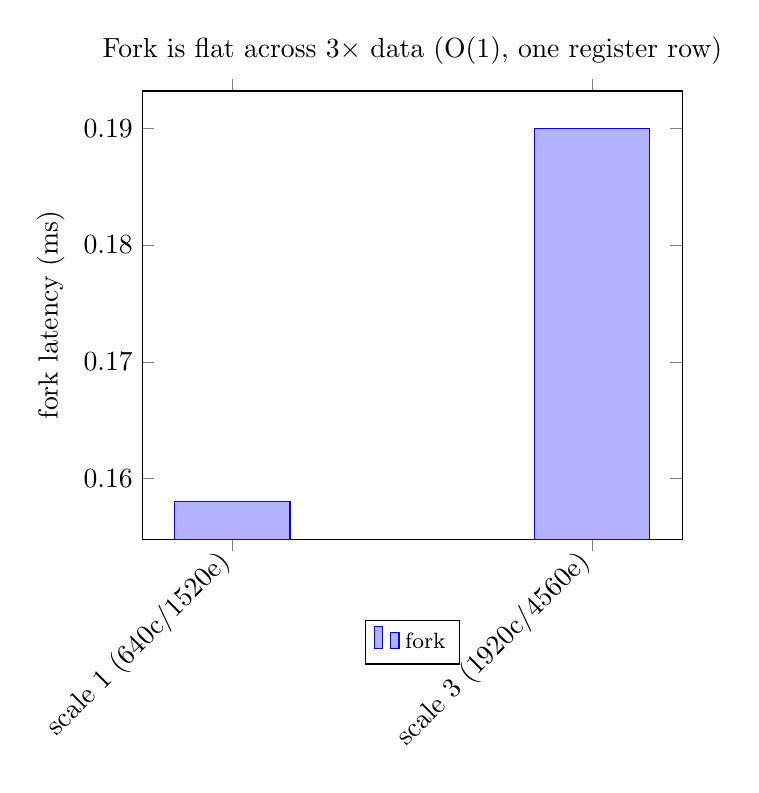
\begin{tikzpicture}
\begin{axis}[
  title={Fork is flat across $3\times$ data (O(1), one register row)},
  ylabel={fork latency (ms)},
  ybar, bar width=0.32,
  enlarge x limits=0.25,
  xtick=data,
  x tick label style={rotate=45,anchor=east},
  xticklabels={{scale 1 (640c/1520e)},{scale 3 (1920c/4560e)}},
  legend style={at={(0.5,-0.18)},anchor=north,legend columns=-1,font=\footnotesize},
  error bars/y dir=both, error bars/y explicit,
]
  \addplot+[error bars/.cd,y explicit] coordinates {
    (1,0.158 ) +- (0,0 )
    (2,0.19 ) +- (0,0 )
  };
  \addlegendentry{fork}
\end{axis}
\end{tikzpicture}
{\footnotesize PRELIMINARY — non-reference hardware; medians of 5, bars show min/max. First readings, not reference figures (paper §5).\par}
